\documentclass[12pt]{article}
\sloppy

\usepackage[utf8]{inputenc}
\usepackage{amsmath, amssymb}
\usepackage{graphicx}
\usepackage{listings}    
\usepackage{hyperref}
\usepackage{float}

\usepackage{booktabs}  % if used in your tables
\usepackage{xcolor}    % if needed for any colored text in tables

\title{Estimating \(\pi\) Value --- Report}
\author{Ranathunga N. D. \\ 200517U}
\date{\today}

\begin{document}

\maketitle

\tableofcontents

\section{Monte Carlo Method: Approach and Implementation}\label{sec:monte-carlo-impl}

The Monte Carlo method for estimating \(\pi\) relies on sampling random points
in \([-1,1]\times[-1,1]\) and counting how many lie within the inscribed
quarter circle:
\[
      \pi \approx 4 \times \frac{\text{Number of points inside the circle}}{\text{Total number of points}}.
\]
A single-threaded approach is excluded due to its long runtime for large
sample sizes. Instead, multi-threaded (pthreads, OpenMP) and GPU-accelerated
(CUDA) implementations are used. The sample size is determined using a
\textbf{binomial} model.

\subsection{Determining Sample Size Using a Binomial Model}\label{sec:bernoulli}
\begin{itemize}
      \item \textbf{Variance Bound:} Each point can be viewed as a Bernoulli trial (success if
            \(\sqrt{x^2 + y^2} \le 1\)), but the total number of successes follows a binomial
            distribution with worst-case variance \(p(1-p)\) with \(p = 0.5\) yields
            \(\sigma^2_{\max} = 0.25\).
      \item \textbf{Samples for Accuracy:}
            \[
                  N \ge \frac{4}{\varepsilon^2}.
            \]
            For \(\varepsilon = 10^{-5}\), \(N \approx 4\times10^{10}\). For \(\varepsilon
            = 10^{-10}\), \(N \approx4\times10^{20}\).
\end{itemize}

\subsubsection{Practical Limit and Diminishing Returns}
\paragraph{Statistical Nature of the Estimator.}
When \(\pi\) is estimated by randomly sampling points in a unit square, the
estimator \(\hat{\pi} = 4 \times (\text{points in circle}/N)\) is unbiased but
has a variance that scales as \(1/N\). By the central limit theorem, its
standard error decreases proportionally to \(1/\sqrt{N}\).

\paragraph{Diminishing Returns on Accuracy.}
Because the error decreases as \(1/\sqrt{N}\):
\begin{itemize}
      \item Doubling \(N\) only reduces the error by about \(1/\sqrt{2}\approx 29\%\).
      \item Each additional decimal place of precision requires roughly 100 times more
            samples.
\end{itemize}

\paragraph{Inherent Random Variance.}
Random fluctuations remain even for large \(N\), diminishing only at the rate
of \(1/\sqrt{N}\). Practical constraints on pseudorandom generation and the
rapid growth in required samples justify fixing the total sample size at
\(\texttt{4} \times 10^{10}\) for the experiments under Question~1.

\subsection{Task Decomposition and Random Number Generation}
\begin{itemize}
      \item \textbf{Common Strategy:} The total sample size \((4 \times 10^{10})\) is divided
            into smaller chunks; each thread (or GPU thread) processes one or more chunks.
            Local counters are maintained to minimize synchronization.
      \item \textbf{Random Numbers:}
            \begin{itemize}
                  \item \(\texttt{std::mt19937}\) (Mersenne Twister) is used with
                        \(\texttt{std::uniform\_real\_distribution}\) over \([-1,1]\).
                  \item Distinct seeds are assigned to each thread to reduce correlation.
            \end{itemize}
      \item \textbf{Data Types:}
            \begin{itemize}
                  \item \(\texttt{unsigned long long}\) is used for counting inside-circle samples.
                  \item \(\texttt{long double}\) is used for storing and returning the final
                        \(\pi\) value.
            \end{itemize}
      \item \textbf{Thread/Block Configuration:}
            \begin{itemize}
                  \item \textbf{CPU Threads:} Up to 12 threads are used on the CPU, as specified
                        by a configuration file.
                  \item \textbf{GPU Threads:} In CUDA, a one-dimensional grid is launched with
                        \(\texttt{threadsPerBlock} = 1024\) and
                        \[
                              \texttt{blocks}
                              = \frac{\texttt{threadCount} + \texttt{threadsPerBlock} - 1}{\texttt{threadsPerBlock}},
                        \]
                        where \(\texttt{threadCount} = 40000\).
            \end{itemize}
\end{itemize}

\subsection{Parallel Implementations: Overview}
\subsubsection{Pthreads-Based Implementation}
\begin{itemize}
      \item \textbf{Thread Creation:} \(\texttt{pthread\_create}\) spawns a fixed number of
            threads, each assigned one or more chunks.
      \item \textbf{Local Counting:} Within each chunk, the condition
            \((x^2 + y^2) \le 1\) is checked. A local counter is incremented whenever a point
            lies inside the circle.
      \item \textbf{Global Summation:} \(\texttt{pthread\_join}\) is used to wait for all
            threads; local counts are then summed to compute the final estimate of \(\pi\).
\end{itemize}

\subsubsection{OpenMP-Based Implementation}
\begin{itemize}
      \item \textbf{Parallel Loop:} A \(\texttt{\#pragma omp parallel for}\) distributes
            chunks among OpenMP threads.
      \item \textbf{Reduction:} A \(\texttt{reduction(+ : totalInsideCount)}\) clause
            accumulates local counters into a global variable.
      \item \textbf{Thread Seeding:} Each thread is assigned a seed offset via
            \(\texttt{omp\_get\_thread\_num()}\).
\end{itemize}

\subsubsection{CUDA-Based Implementation}
\begin{itemize}
      \item \textbf{Kernel Launch:} A kernel (\(\texttt{MCKernel}\)) is invoked with the chosen
            block and thread configuration. Each GPU thread processes a portion of the samples.
      \item \textbf{curand\_init:} Each thread initializes a local PRNG state, generating points
            in \([-1,1]\times[-1,1]\).
      \item \textbf{Atomic Accumulation:} Each thread’s local count is added to a global counter
            using \(\texttt{atomicAdd}\). The final count is copied back to the CPU.\@
\end{itemize}

\subsection{Hardware Specifications}
\begin{table}[h]
      \centering
      \begin{tabular}{ll}
            \toprule
            \textbf{CPU Model}     & Intel (R) Core (TM) i7--9750H CPU @ 2.60GHz \\
            \textbf{Cores/Threads} & 6 Cores / 12 Threads                        \\
            \textbf{RAM}           & 16\,GiB DDR4                                \\
            \midrule
            \textbf{GPU Model}     & NVIDIA GeForce (CUDA Version 11.4)          \\
            \textbf{GPU Memory}    & 3911\,MiB                                   \\
            \bottomrule
      \end{tabular}
      \caption{Summary of CPU and GPU hardware used in the experiments.}\label{tab:hardware}
\end{table}

\subsection{Implementation Details}
\begin{itemize}
      \item \textbf{Time Measurement:} The total runtime is measured using
            \(\texttt{std::chrono::high\_resolution\_clock}\). The start time is recorded
            immediately before the estimation begins, and the end time is recorded after
            all threads (or GPU kernels) have completed.
      \item \textbf{Compilation:} A \(\texttt{CMakeLists.txt}\) file and a Makefile are used
            to compile and run the code, though these details do not affect the methodology
            directly.
\end{itemize}

\section{Part A\texorpdfstring{\@:}{:} Experimental Tasks and Results}

\subsection{Task A.1: Evaluating \texorpdfstring{\(\pi\)}{pi} to Different Decimal Places}

\begin{table}[H]
\centering
\caption{Precision-based results for Pthreads}
\label{tab:pthreads-precision}
\begin{tabular}{|l|l|l|}
\hline
Precision & Pi Estimate & Time (s) \\
\hline
5 & 3.14159 & 233.626 \\
10 & 3.1415886455 & 238.334 \\
15 & 3.141602155100000 & 232.330 \\
20 & 3.14158805580000000004 & 231.193 \\
\hline
\end{tabular}
\end{table}

\begin{table}[H]
\centering
\caption{Precision-based results for OpenMP}
\label{tab:openmp-precision}
\begin{tabular}{|l|l|l|}
\hline
Precision & Pi Estimate & Time (s) \\
\hline
5 & 3.14159 & 244.388 \\
10 & 3.1415845871 & 249.834 \\
15 & 3.141601863300000 & 242.200 \\
20 & 3.14158336399999999996 & 239.260 \\
\hline
\end{tabular}
\end{table}

\begin{table}[H]
\centering
\caption{Precision-based results for CUDA}
\label{tab:cuda-precision}
\begin{tabular}{|l|l|l|}
\hline
Precision & Pi Estimate & Time (s) \\
\hline
5 & 3.14158 & 9.036 \\
10 & 3.1415923941 & 8.762 \\
15 & 3.141592781500000 & 8.786 \\
20 & 3.14158480229999999994 & 8.786 \\
\hline
\end{tabular}
\end{table}


\subsection{Task A.2: Reassessing Strategies for Specific Trial Counts}
\begin{table}[H]
\centering
\caption{$2^n$-based results for Pthreads}
\label{tab:pthreads-2n}
\begin{tabular}{|l|l|l|l|l|}
\hline
Experiment & Total Samples & Pi Estimate & Time (s) & Error \\
\hline
$2^{24}$ trials & 16777216 & 3.14161205291748046875 & 0.094 & 0.000019 \\
$2^{26}$ trials & 67108864 & 3.14167696237564086914 & 0.520 & 0.000084 \\
$2^{28}$ trials & 268435456 & 3.14164182543754577637 & 1.794 & 0.000049 \\
\hline
\end{tabular}
\end{table}

\begin{table}[H]
\centering
\caption{$2^n$-based results for OpenMP}
\label{tab:openmp-2n}
\begin{tabular}{|l|l|l|l|l|}
\hline
Experiment & Total Samples & Pi Estimate & Time (s) & Error \\
\hline
$2^{24}$ trials & 16777216 & 3.14237880706787109375 & 0.083 & 0.000786 \\
$2^{26}$ trials & 67108864 & 3.14174300432205200195 & 0.450 & 0.000150 \\
$2^{28}$ trials & 268435456 & 3.14153531193733215332 & 1.867 & 0.000057 \\
\hline
\end{tabular}
\end{table}

\begin{table}[H]
\centering
\caption{$2^n$-based results for CUDA}
\label{tab:cuda-2n}
\begin{tabular}{|l|l|l|l|l|}
\hline
Experiment & Total Samples & Pi Estimate & Time (s) & Error \\
\hline
$2^{24}$ trials & 16777216 & 3.13798832893371582031 & 0.004 & 0.003604 \\
$2^{26}$ trials & 67108864 & 3.14036542177200317383 & 0.016 & 0.001227 \\
$2^{28}$ trials & 268435456 & 3.14094561338424682617 & 0.060 & 0.000647 \\
\hline
\end{tabular}
\end{table}


\subsection{Task A.3: Profiling the Best-Performing Program}
After running the experiments, the GPU-based Monte Carlo approach was
identified as the best performer for large-scale sampling. Profiling was
performed using Nsight Compute (\texttt{ncu}), and the following key
observations were made:

\paragraph{Warp Stall Sampling.}
\begin{figure}[ht]
      \centering
      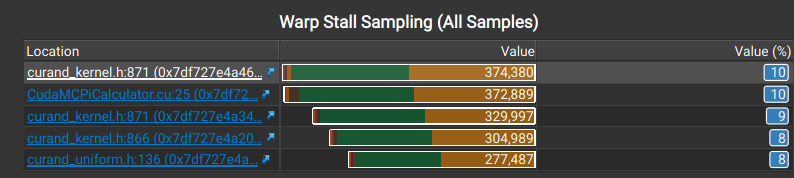
\includegraphics[width=0.7\textwidth]{images/stalls.png}
      \caption{Warp Stall Sampling view}\label{fig:warp-stalls}
\end{figure}
Figure~\ref{fig:warp-stalls} shows that functions in \texttt{curand\_kernel.h}
account for significant warp stalls (10\% each for two instances), with
\texttt{CudaMCPiCalculator.cu} also registering around 8\%--9\% of stalls.
These stalls are primarily related to random number generation and the
\texttt{if (x * x + y * y <= 1.0f)} check within the kernel.

\paragraph{Instruction-Level Analysis.}
\begin{figure}[ht]
      \centering
      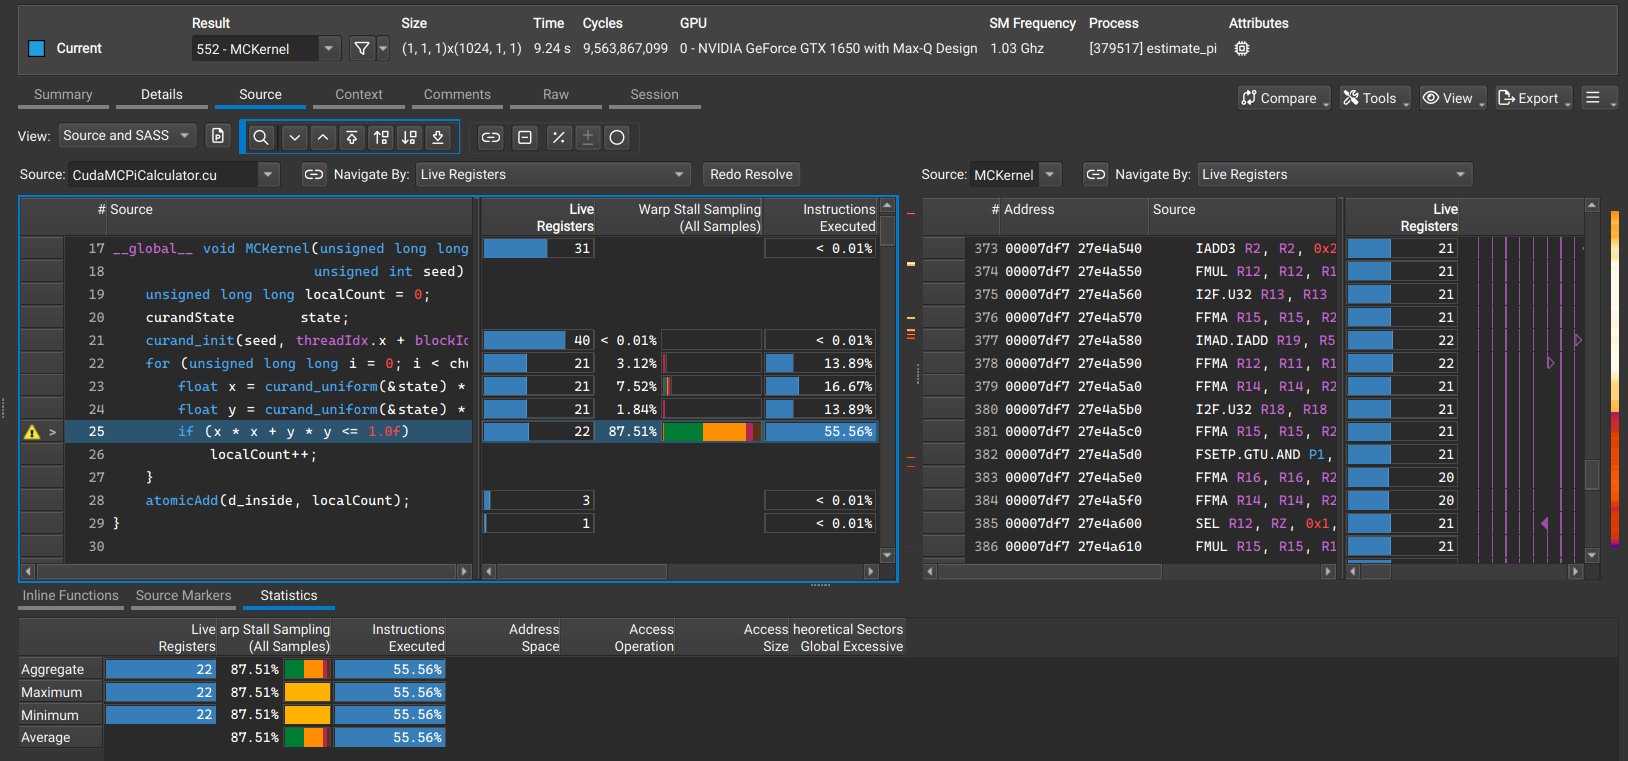
\includegraphics[width=0.9\textwidth]{images/warp-stalls.png}
      \caption{Source and SASS Analysis}\label{fig:kernel-instructions}
\end{figure}
Figure~\ref{fig:kernel-instructions} indicates that the conditional check
\texttt{if (x * x + y * y <= 1.0f)} causes a significant share of warp stalls.
In a GPU’s SIMT (Single Instruction, Multiple Threads) architecture, threads
are grouped into warps that execute the same instruction in lockstep. When a
branching instruction (like an \texttt{if}-statement) occurs, some threads may
take one path while others take another, leading to \emph{divergence}. Divergent
warps must serialize the execution of each path, which stalls threads on the
inactive path. This serialization can reduce overall throughput, especially
when the conditional is evaluated many times per thread. Although the distance
check is essential for the Monte Carlo approach, reducing divergence can mitigate
these stalls.

\paragraph{Pipe Utilization.}
\begin{figure}[ht]
      \centering
      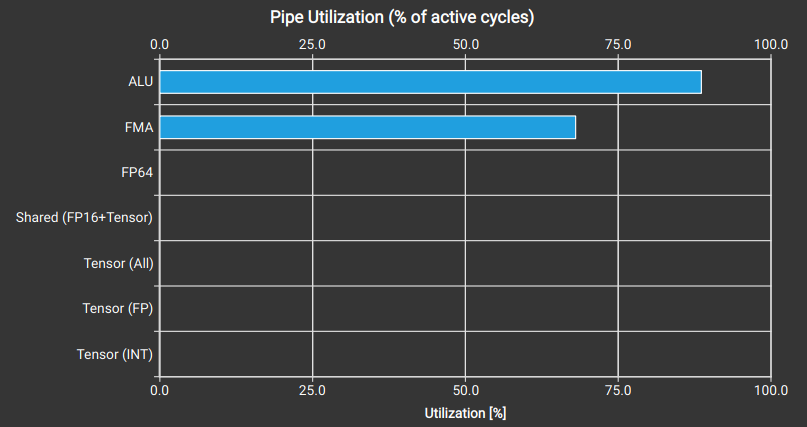
\includegraphics[width=0.7\textwidth]{images/pipe-utilization.png}
      \caption{Pipe utilization}\label{fig:pipe-util}
\end{figure}
Figure~\ref{fig:pipe-util} presents the pipe utilization. The ALU is utilized
most heavily, followed by the FMA (fused multiply-add) units. This is expected
given the arithmetic nature of the distance check \((x^2 + y^2)\) and other
basic floating-point operations.

\paragraph{Memory Chart.}
\begin{figure}[ht]
      \centering
      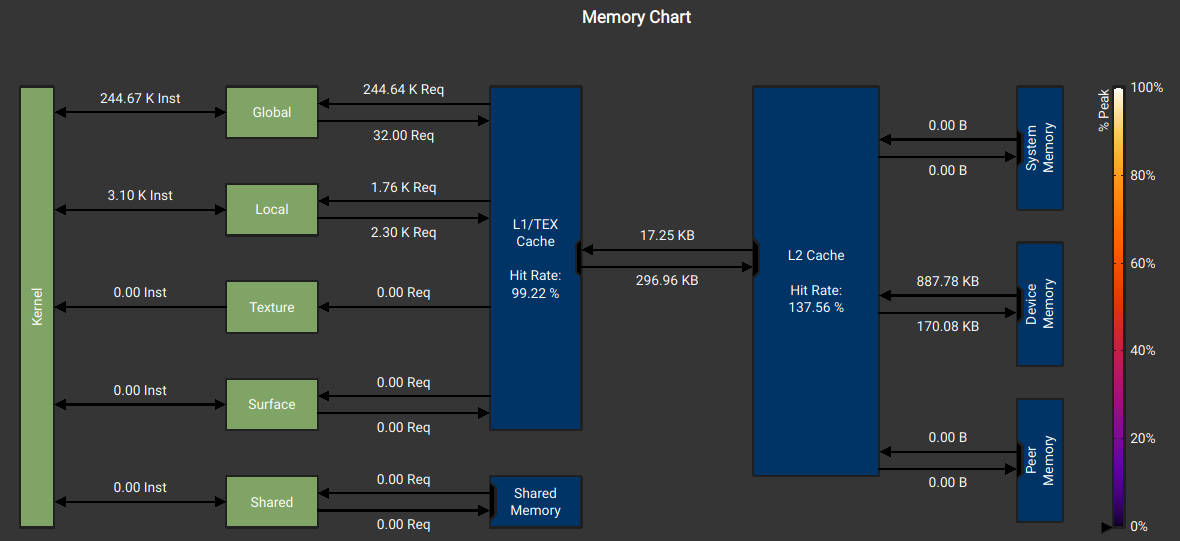
\includegraphics[width=0.8\textwidth]{images/memory-chart.png}
      \caption{Memory chart}\label{fig:memory-chart}
\end{figure}
Figure~\ref{fig:memory-chart} shows the memory chart. Global memory requests
are relatively small, since only a single atomic addition is performed per
thread block (to accumulate the inside-circle count). Consequently, the memory
subsystem does not appear to be a major bottleneck. L2 cache hit rates are high,
and only minimal data is transferred between host and device, so bandwidth is
not saturated.

\paragraph{Potential Optimizations.}
\begin{itemize}
      \item \textbf{Random Number Generation Bottleneck:} The \texttt{curand\_kernel.h}
            calls introduce warp stalls. More efficient RNG strategies or caching random
            values in shared memory could reduce this overhead.
      \item \textbf{Conditional Check Overhead:} The \texttt{if ($x^2 + y^2 \le 1.0f$)}
            line is repeatedly executed. While unavoidable, exploring warp-level
            primitives or reducing divergence may help.
      \item \textbf{Memory System:} Memory bandwidth is not saturated, so optimizing
            global memory usage is less critical. However, a shared-memory reduction
            might still reduce atomic overhead.
\end{itemize}

\subsection{Task A.4: Discussion of Findings and Limitations}

\paragraph{Accuracy.}
Monte Carlo methods are probabilistic; achieving precision beyond a few decimal
places quickly becomes expensive due to the \(1/\sqrt{N}\) error scaling. Each
additional digit of accuracy necessitates roughly 100 times more samples.

\paragraph{Profiling Insights.}
Profiling the GPU code revealed that:
\begin{itemize}
      \item \texttt{curand\_kernel.h} introduces significant warp stalls due to random
            number generation.
      \item Repeated distance checks \((x^2 + y^2 \le 1)\) also stall warps, though they
            are unavoidable for this approach.
      \item Memory usage is minimal, so bandwidth is not a bottleneck.
\end{itemize}

\paragraph{Limitations.}
\begin{itemize}
      \item \textbf{Randomness Quality:} The estimator depends on good pseudorandom generation.
      \item \textbf{Complexity:} Threading libraries and CUDA kernels add development overhead.
\end{itemize}

\section{Part B: Gregory-Leibniz Series for \texorpdfstring{\(\pi\)}{pi}}
The Gregory-Leibniz series for \(\pi\) is given by:
\[
      \pi = 4 \sum_{n=0}^{\infty} \frac{(-1)^n}{2n + 1}.
\]
\subsection{Implementation and Observations}
\begin{itemize}
      \item \textbf{Implementation}: A dynamic approach was used, where the kernel-based
            summation accumulates terms until a specified decimal precision is reached.
            This eliminates random variance but requires explicit tracking of convergence.
      \item \textbf{Convergence}: The series converges relatively slowly compared to some
            other infinite series for \(\pi\). However, it still tends to require fewer
            terms for a given precision than a Monte Carlo approach needs samples,
            especially as precision grows.
      \item \textbf{Comparison to Monte Carlo}:
            \begin{itemize}
                  \item \textbf{Monte Carlo’s High Sample Requirements}: Achieving
                        high-precision estimates with Monte Carlo generally demands an
                        exponentially larger number of random samples, leading to slow
                        convergence for many-decimal-place accuracy.
                  \item \textbf{Parallelization Ease}: Monte Carlo is straightforward to
                        parallelize (each sample is independent), whereas Gregory-Leibniz
                        requires careful summation of partial results. Nonetheless, both can
                        benefit from multi-threading or GPU kernels.
                  \item \textbf{Deterministic vs. Stochastic}: Gregory-Leibniz produces
                        deterministic results without random variance, whereas Monte Carlo
                        is inherently probabilistic.
            \end{itemize}
\end{itemize}

\subsection{Experimental Results and Comparison}
\begin{table}[H]
      \centering
      \caption{Gregory-Leibniz GPU Results (Dynamically Terminated)}\label{tab:gregory-leibniz-results}
      \begin{tabular}{|l|l|l|} % @{}rlll@{}
            \hline
            \textbf{Precision} & \textbf{Pi Estimate} & \textbf{Time (s)} \\
            \hline
            5                  & 3.14159              & 1.765             \\
            6                  & 3.141592             & 3.934             \\
            7                  & 3.1415924            & 11.876            \\
            8                  & 3.14159255           & 36.433            \\
            9                  & 3.141592622          & 120.241           \\
            10                 & 3.1415926436         & 394.454           \\
            \hline
      \end{tabular}
\end{table}

\paragraph{Time Comparison with Monte Carlo.}
\begin{itemize}
      \item \textbf{Precision vs. Performance}: The Monte Carlo approach requires
            a rapidly growing number of samples to reach higher decimal places, often
            making it slower than Gregory-Leibniz for equivalent precision. By contrast,
            the Gregory-Leibniz series, though still slow, can achieve a target precision
            with fewer total operations than a naive Monte Carlo at very high decimal places.
      \item \textbf{Parallel Scalability}: Monte Carlo is conceptually simpler to
            parallelize (each sample is independent), but the overhead of generating
            large numbers of samples can still be high. Gregory-Leibniz parallelization
            involves summing partial results, yet each iteration is deterministic and
            free of variance.
\end{itemize}

\section*{Conclusion}
In summary, the Monte Carlo and Gregory-Leibniz methods each provide valid
approaches to estimating \(\pi\). Monte Carlo is conceptually simple to parallelize
but requires a rapidly growing number of samples for higher precision. The
Gregory-Leibniz series converges deterministically, often requiring fewer total
iterations at very high precision, though it still grows slowly and demands
careful summation for parallel performance. Ultimately, the choice depends on
available hardware, desired accuracy, and implementation complexity.

\end{document}
